% Author: Izaak Neutelings (July 2018)
\documentclass[border=3pt,tikz]{standalone}
\usepackage{amsmath}
\usepackage{tikz}
%\usetikzlibrary{fpu}
%\usepackage[autolanguage]{numprint}
\tikzset{>=latex} % for LaTeX arrow head
\tikzstyle{axis}=[->,thick,black]
\tikzstyle{tick}=[thick,black]
\pgfkeys{/pgf/number format/precision=2}



\begin{document}
\Large



% 1D SCAN
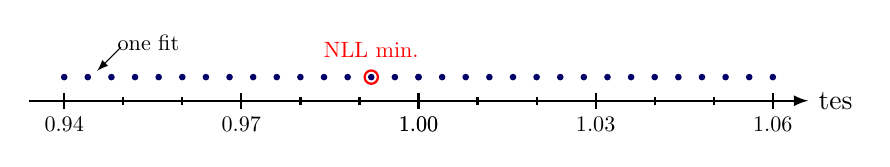
\begin{tikzpicture}
  \def\s{75} % scale
  \def\tmax{0.06}
  \def\xmax{\tmax*\s} % axis length
  \def\Nticks{6} % number of ticks
  \def\nticks{2} % number of small ticks
  \def\l{0.05} % small tick length
  \def\L{0.10} % large tick length
  \def\N{15} % number of points
  \def\R{1.2pt}
  
  % AXES
  \draw[axis] (-1.1*\xmax,0) -- (+1.1*\xmax,0) node[right] {tes}; %{$\text{tes}$};  
  \foreach \i [evaluate={\x=\i*\xmax/\Nticks;
                         \tesU=1.0+\i*\tmax/\Nticks; \tesD=1.0-\i*\tmax/\Nticks;
                         \c=(mod(\i,\nticks+1)==0);}] in {0,...,\Nticks}{
    \if\c1
      \draw[tick] (+\x,+\L) -- (+\x,-\L) node[below,scale=0.8] {\pgfmathroundtozerofill{\tesU}\pgfmathresult};
      \draw[tick] (-\x,+\L) -- (-\x,-\L) node[below,scale=0.8] {\pgfmathroundtozerofill{\tesD}\pgfmathresult};
    \else
      \draw[tick] (+\x,+\l) -- (+\x,-\l);
      \draw[tick] (-\x,+\l) -- (-\x,-\l);
    \fi
  }
  
  % DOTS
  \foreach \i [evaluate={\x=\i*\xmax/\N;}] in {0,...,\N}{
    \fill[black!60!blue] (+\x,3*\L) circle (\R);
    \fill[black!60!blue] (-\x,3*\L) circle (\R);
  }
  \draw[<-] ({-(\N-1.4)*\xmax/\N},3.8*\L) --++ (3*\L,3*\L) node[above right=-4,scale=0.8] {one fit};
  \draw[tick,red] (-2*\xmax/\N,3*\L) circle (2*\R) node[above=4,scale=0.8] {NLL min.};
  
  
\end{tikzpicture}



% 2D SCAN
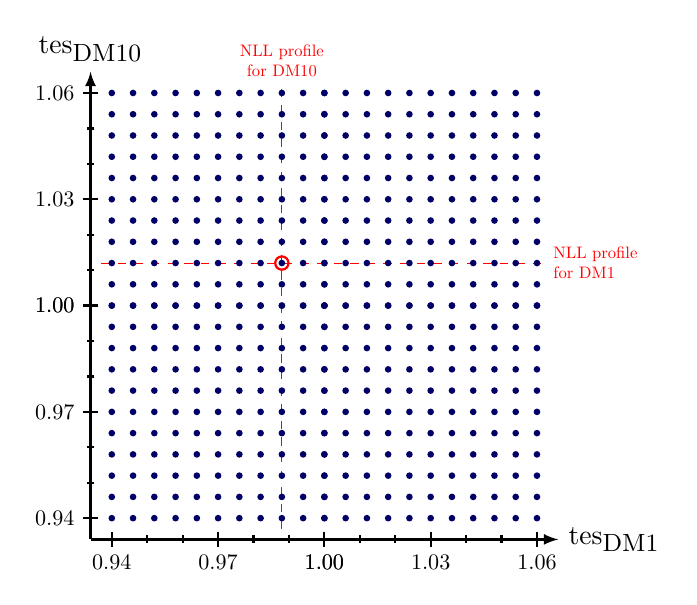
\begin{tikzpicture}
  \def\s{45} % scale
  \def\tmax{0.06}
  \def\xmax{\tmax*\s} % axis length
  \def\y{-1.1*\xmax} % axis zero
  \def\Nticks{6} % number of ticks
  \def\nticks{2} % number of small ticks
  \def\l{0.05} % small tick length
  \def\L{0.10} % large tick length
  \def\N{10} % number of points
  \def\R{1.2pt}
  
  % AXES
  \draw[axis] (-1.1*\xmax,\y) -- (+1.1*\xmax,\y) node[right] {$\text{tes}_\text{\small DM1}$};  
  \draw[axis] (\y,-1.1*\xmax) -- (\y,+1.1*\xmax) node[above] {$\text{tes}_\text{\small DM10}$};  
  \foreach \i [evaluate={\x=\i*\xmax/\Nticks;
                         \tesU=1.0+\i*\tmax/\Nticks; \tesD=1.0-\i*\tmax/\Nticks;
                         \c=(mod(\i,\nticks+1)==0);}] in {0,...,\Nticks}{
    \if\c1
      \draw[tick] (+\x,\y+\L) -- (+\x,\y-\L) node[below,scale=0.8] {\pgfmathroundtozerofill{\tesU}\pgfmathresult};
      \draw[tick] (-\x,\y+\L) -- (-\x,\y-\L) node[below,scale=0.8] {\pgfmathroundtozerofill{\tesD}\pgfmathresult};
      \draw[tick] (\y+\L,+\x) -- (\y-\L,+\x) node[left,scale=0.8] {\pgfmathroundtozerofill{\tesU}\pgfmathresult};
      \draw[tick] (\y+\L,-\x) -- (\y-\L,-\x) node[left,scale=0.8] {\pgfmathroundtozerofill{\tesD}\pgfmathresult};
    \else
      \draw[tick] (+\x,\y+\l) -- (+\x,\y-\l);
      \draw[tick] (-\x,\y+\l) -- (-\x,\y-\l);
      \draw[tick] (\y+\l,+\x) -- (\y-\l,+\x);
      \draw[tick] (\y+\l,-\x) -- (\y-\l,-\x);
    \fi
  }
  
  % DOTS
  \draw[dashed,red]
    (-1.05*\xmax,+2*\xmax/\N) -- (+1.05*\xmax,+2*\xmax/\N)
    node[right,scale=0.6,align=left] {NLL profile\\for DM1};
  \draw[dashed,red]
    (-2*\xmax/\N,-1.05*\xmax) -- (-2*\xmax/\N,+1.05*\xmax)
    node[above,scale=0.6,align=center] {NLL profile\\for DM10};
  \foreach \i [evaluate={\x=\i*\xmax/\N;}] in {0,...,\N}{
    \foreach \i [evaluate={\y=\i*\xmax/\N;}] in {0,...,\N}{
      \fill[black!60!blue] (+\x,\y) circle (\R);
      \fill[black!60!blue] (-\x,\y) circle (\R);
      \fill[black!60!blue] (+\x,-\y) circle (\R);
      \fill[black!60!blue] (-\x,-\y) circle (\R);
    }
  }
  \draw[tick,red] (-2*\xmax/\N,+2*\xmax/\N) circle (2*\R);
  
\end{tikzpicture}




\end{document}